\documentclass[12pt, letterpaper]{article}
\usepackage{graphicx} % Required for inserting images
\usepackage{authblk} % Dos autores o más
\usepackage[spanish]{babel}
\usepackage{caption}
\usepackage{subcaption}
\usepackage{multicol}

\title{\textbf{Estructura del documento}}
\author[1]{Manuel Olmos Antillón}
\author[2]{\\Ximena Serna Mendoza}
\author[2]{\\Guillermo Ian Barbosa Martínez}
\author[3]{\\Ismael Posadas Pichardo}
\author[4]{\\Paolo Medrano Magaña}
\affil[1]{Ingeniería en Sistemas Computacionales, Escuela de Ingeniería y Ciencias, Tecnológico de Monterrey}
\affil[2]{Ingeniería en Ciencia de Datos y Matemáticas, Escuela de Ingeniería y Ciencias, Tecnológico de Monterrey}
\affil[3]{Ingeniería en Nanotecnología, Escuela de Ingeniería y Ciencias, Tecnológico de Monterrey}
\affil[4]{Ingeniería en Biotecnología, Escuela de Ingeniería y Ciencias, Tecnológico de Monterrey}

\date{\today}

\begin{document}

\maketitle
\newpage

\begin{abstract}
here you have to write the abstract
\end{abstract}

\tableofcontents
\section{Introducción}

Este reporte representa la culminación de un proyecto dedicado a modelar en \textit{Python} al \textit{Rover Perseverance} de la NASA \cite{meeker2021twin}, enfocado en su exploración en busca de agua en Marte \cite{campo2022clasificacion}. A lo largo de diversas entregas, hemos abordado la adaptación de conceptos clave de la inteligencia artificial, como el modelo PEAS, y la aplicación de una variedad de algoritmos de búsqueda, tanto informada como no informada, para analizar su eficiencia en un entorno simulado. Se ha abordado desde la revisión inicial de la misión del \textit{Perseverance} y la descripción de su entorno, hasta el análisis detallado de algoritmos de búsquedas informadas (\textit{greedy}, costo uniforme y A*), no informadas (anchura y profundidad) y locales (\textit{hill climbing}, \textit{hill climbing with random restarts} y \textit{simulated annealing} ó recocido simulado \cite{banchs1997simulated}), y se ha explorado cómo este agente inteligente aborda su tarea en un ambiente desafiante como el marciano. En este informe, se consolidarán los hallazgos y conclusiones obtenidos a lo largo de cada etapa de este proyecto, ofreciendo una visión integral del desempeño y las capacidades del \textit{Rover Perseverance} \cite{luc1990cooperation} en su búsqueda de agua en Marte.

\section{PEAS}

    \subsection{Performance}\label{performance}

    Como se comentó anteriormente, en esta situación el agente es un robot explorador conocido como \textit{Rover Perseverance}. De acuerdo con la NASA, esta entidad es capaz de recolectar muestras de roca y regolito con base en evaluaciones de sus características químicas, físicas, minerales y orgánicas en búsqueda de signos de vida microbiana antigua \cite{carlos2023factores, bell2021mars}. De esta manera, se espera que las almacene y, posteriormente, las deposite sobre superficie marciana para ser recuperadas en una misión futura para ser analizadas en grandes laboratorios aquí en la Tierra.
    
    \subsection{Environment}\label{environment}

    El ambiente del robot es el cráter de Jezero en Marte. Es una región cuyo entorno antiguo, según la NASA, pudo haber favorecido la vida microbiana, lo que podría indicar la posibilidad de que existiera la presencia de agua o viscosidad, así como otros factores como la presencia de otros nutrientes, la humedad de la región misma, junto con otras características físicas, químicas, minerales, etc. Además, el cráter, como se ha podido observar en los registros de las recolecciones de la misión, cuenta con rocas marcianas que pueden ser útiles para análisis exhaustivos posteriores.
    
        \subsubsection{¿Accesible o inaccesible?}

        \textbf{85\% accesible}: el \textit{Perseverance} cuenta con tecnología de punta. Más adelante se hablará sobre esto. Bajo la lupa geológica, algunos factores potenciales para el estudio de vida en el cráter de Jezero, como la composición y estructura internas de la región, son límites naturales del \textit{Rover} debido a la complejidad de estos instrumentos y herramientas que ya de por sí en nuestro planeta representan. Esto va de la mano también con el acceso más microscópico a las estructuras físicas, químicas, etc. de las formas de vida a estudiar. Esto se puede justificar argumentando que el objetivo del \textit{Rover} es, ante todo, la recolección de estos “artículos” para una futura misión de recuperación de estos materiales para un análisis posterior y mucho más sofisticado con herramientas tecnológicas en laboratorios mucho más revolucionarias.
    
        \subsubsection{¿Determinista o No determinista?}

        \textbf{60\% determinista}: Dados los conocimientos actuales sobre Marte, así como las determinadas rutinas o actividades de exploración sobre el cráter de Jezero específicamente, se pueden determinar numerosos estados futuros e importantes en el cráter. No obstante, es precisamente este factor de incertidumbre, así como comportamientos o fenómenos del planeta que aún podrían ser desconocidos para nosotros \cite{pardo2020geologia}. Además, eventos como las conocidas tormentas de polvo contribuyen a la aleatoriedad a la que se enfrenta el \textit{Rover} en este ambiente.
        
        \subsubsection{¿Episódico o No episódico?}

        \textbf{No episódico}: El cráter de Jezero en Marte no cuenta con procesos bien definidos por inicio o final. A pesar de que pueden tener lugar numerosas acciones y percepciones por parte del agente, su entorno no le permite establecer períodos bien definidos y conocidos, más allá de procesos de exploración, análisis y descubrimiento que tampoco tienen momentos con inicio o fin bien constituidos en el entorno.
        
        \subsubsection{¿Estático o dinámico?}

        \textbf{95\% estático}: a pesar de la aleatoriedad e incertidumbre que aún puede rodear a la región a explorar, por lo general se entiende como monótono y desértico al entorno que encierra al cráter. Dada la escasa actividad geológica, la falta de evidencia sólida de la presencia de agua en la actualidad y las bajas temperaturas del planeta, sugieren que en realidad tanto el cráter como el planeta presentan muy poca actividad. La incertidumbre radica principalmente en los mencionados fenómenos del planeta rojo que aún podría ser desconocidos para nosotros o el agente, así como los conocidos como las tormentas de polvo.
    
        \subsubsection{¿Discreto o continuo?}

        \textbf{Continuo}: Es irónico que, pese al ya mencionado carácter desértico de Marte, como se ha comentado anteriormente, existan procesos ya conocidos. En esta ocasión, hay uno en particular que indica una producción constante de un gas vital para procesos geológicos. Se trata del metano que, aunque no es prueba contundente de la existencia de vida microbiana, sugiere junto con otros factores de disciplinas científicas mencionadas como la geología, la química y la física, actividad en el planeta. Esta actividad, además de la generación de gas metano, puede ir desde los climas de Marte, su recepción de peligrosa radiación cósmica \cite{campillo2021arquitecturas}, etc. sugieren la carencia de un número o patrón bien definido de acciones y, ahora con el agente, percepciones que pueden verse en el planeta rojo.
    
    \subsection{Actuators}\label{actuators}

        \begin{itemize}

            \item Ruedas para moverse y desplazarse a lo largo del cráter.
            \item Trípode integrado a la cámara que le permite moverse también y tener vista panorámica.
            \item Láser ultravioleta, integrado al receptor SHERLOC para hallar químicos.
            \item MOXIE\cite{hoffman2022mars}, que produce oxígeno a raíz del dióxido de carbono de la atmósfera del planeta. Es también sensor, ya que debe detectar el químico y transformarlo.
            \item Láseres para disparar a rocas marcianas bien identificadas.
            \item Tubos de ensayo de titanio que almacenan rocas marcianas para análisis posteriores.
            \item Taladro de perforación para horadar la superficie marciana y depositar los tubos.
            \item Brazo que cuenta con el taladro y le da dirección a este, además de que permite sujetar cuidadosamente las muestras para almacenarlas, depositarlas, etc.
            \item Chasis que sirve para guardar los tubos que almacenen muestras importantes.
        
        \end{itemize}
    
    \subsection{Sensors}\label{sensors}

        \begin{itemize}

            \item SuperCam\cite{maurice2021supercam}, un cámara con tecnología de punta que permite al robot ver a increíbles distancias identificar químicos.
            \item Micrófono, que permite no solo que el robot escuche, sino que registre en audio procesos como al robot mismo desplazándose, el aire del planeta, los impactos del láser a rocas marcianas, etc.\cite{leighton2021thoughts}
            \item SHERLOC\cite{beegle2016sherloc} y el láser ultravioleta que tienen incorporado. A pesar de que le permite al agente actuar de determinada manera para buscar objetos, también le permite sentirlos, detectarlos, y obtener información del entorno con base en ello.
            \item RIMFAX\cite{hamran2015rimfax}: un espectrómetro con rayos X que, prácticamente, permite al \textit{Rover} ver bajo la superficie con un georadar en busca de características geológicas.
            \item PIXL\cite{allwood2021pixl}: otro espectrómetro con rayos X y cámara que permite al agente medir la composición química de las rocas a una escala muy fina e incluso tomarles foto a estas y a las texturas del suelo marciano.
            \item MOXIE: su papel como sensor radica en la detección de dióxido de carbono. Por otro lado, como se comentó en el apartado anterior, su rol como actuador es producir oxígeno propio. Es una prueba para futuros exploradores.
        s
        \end{itemize}

\section{Representaciones}

    \begin{table}[h!]
        \centering
        \begin{tabular}{|c|c|} % chktex 44
            \hline % chktex 44
            \textbf{Elemento} & \textbf{Símbolo} \\
            \hline % chktex 44
            Agua & -\\
            \hline % chktex 44
            Obstáculos & * \\
            \hline % chktex 44
            Niveles topográficos & 1, 2, 3, 4, 5, 6 \\
            \hline % chktex 44
            Límite del terreno & \# \\
            \hline % chktex 44
            Rover & + \\
            \hline % chktex 44
        \end{tabular}
        \caption{Representaciones de los elementos en el mapa.}
        \label{tabla:representaciones}
    \end{table}

\section{Modelos generados}

    \begin{figure}[h!]
        \centering
        \begin{subfigure}[h!]{0.45\textwidth}
            \centering
            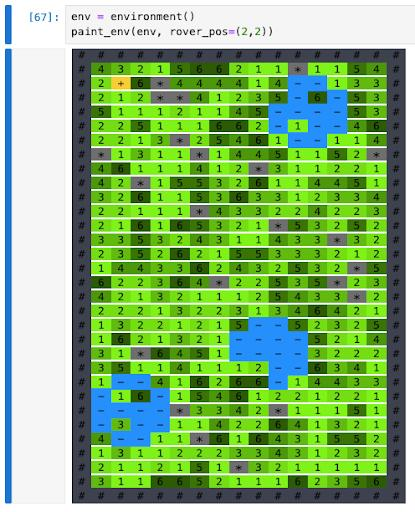
\includegraphics[scale=0.25,angle=0]{env.jpeg}
        \end{subfigure}
        \hfill
        \centering
        \caption{Primera prueba de generación de un mundo aleatoria para el \textit{Rover Perseverance}}
        \label{env}
    \end{figure}

    \begin{figure}[h!]
        \centering
        \begin{subfigure}[h!]{0.45\textwidth}
            \centering
            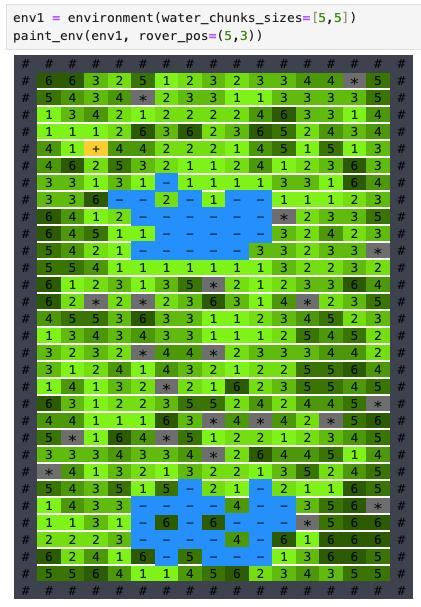
\includegraphics[scale=0.25,angle=0]{env1.jpeg}
        \end{subfigure}
        \hfill
        \centering
        \caption{Segunda prueba de generación de un mundo aleatoria para el \textit{Rover Perseverance}}
        \label{env1}
    \end{figure}

    \begin{figure}[h!]
        \centering
        \begin{subfigure}[h!]{0.45\textwidth}
            \centering
            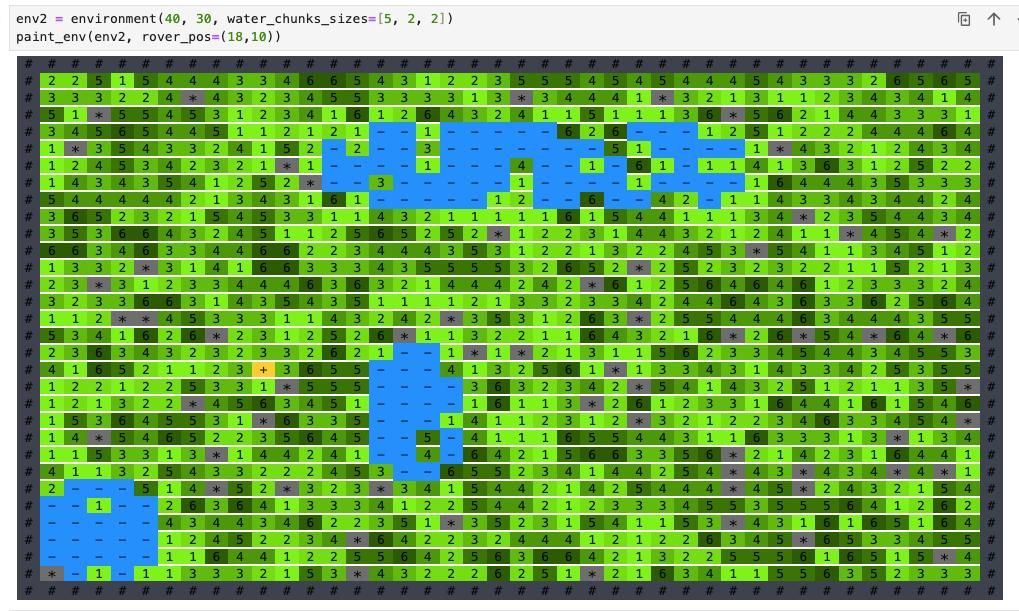
\includegraphics[scale=0.16,angle=0]{env2.jpeg}
        \end{subfigure}
        \hfill
        \centering
        \caption{Tercera prueba de generación de un mundo aleatoria para el \textit{Rover Perseverance}}
        \label{env2}
    \end{figure}

\section{Evidencia de funcionamiento}

\section{Documentación del Programa en Python}

El código \textit{environment} contiene una serie de funciones que permiten crear un mapa con cuerpos de agua, obstáculos y terreno de variadas alturas de manera aleatoria, buscando generar una representación plausible de un entorno natural.

Las funciones implementadas otorgan al usuario la libertad de especificar la cantidad y tamaños de los cuerpos de agua, cantidad de obstáculos, altura máxima de terreno, etc.

    \subsection{Librerías}
        \paragraph{\textit{random}}
        \cite{abdugafforovna2023modules} Para la generación de coordenadas y dimensiones aleatorias apegadas a los requisitos proporcionados para el reto.

        \paragraph{\textit{SimpleAI}}
        \cite{thaker2020python} Para ejecutar algoritmos de búsqueda informadas, no informadas y locales para el agente diseñado.

    \subsection{Funciones}

        \subsubsection{\textit{init\_env (width, height)}}

            \paragraph{Recibe}
            \dots
            \paragraph{Regresa}
            \dots
            \paragraph{Descripción}

        \subsubsection{\textit{square\_coordinates (top\_corner, bottom\_corner, circular)}}

            \paragraph{Recibe}
            \dots
            \paragraph{Regresa}
            \dots
            \paragraph{Descripción}

        \subsubsection{\textit{generate\_water\_chunks (env, water\_chunks\_sizes, percentages)}}

            \paragraph{Recibe}
            \dots
            \paragraph{Regresa}
            \dots
            \paragraph{Descripción}

        \subsubsection{\textit{generate\_obstacles (env, obstacles, percentages)}}

            \paragraph{Recibe}
            \dots
            \paragraph{Regresa}
            \dots
            \paragraph{Descripción}

        \subsubsection{\textit{surrounding (env, coordinate)}}

            \paragraph{Recibe}
            \dots
            \paragraph{Regresa}
            \dots
            \paragraph{Descripción}

        \subsubsection{\textit{generate\_terrain (env, max\_terrain\_height)}}

            \paragraph{Recibe}
            \dots
            \paragraph{Regresa}
            \dots
            \paragraph{Descripción}

        \subsubsection{\textit{generate\_border (env)}}

            \paragraph{Recibe}
            \dots
            \paragraph{Regresa}
            \dots
            \paragraph{Descripción}

        \subsubsection{\textit{remove\_border (env)}}

            \paragraph{Recibe}
            \dots
            \paragraph{Regresa}
            \dots
            \paragraph{Descripción}

        \subsubsection{\textit{environment (width, height, water\_chunks\_sizes, w\_sizes\_percentage, obstacles, o\_size\_percentage, max\_terrain\_height, add\_border)}}

            \paragraph{Recibe}
            \dots
            \paragraph{Regresa}
            \dots
            \paragraph{Descripción}

        \subsubsection{\textit{paint\_env (env, show\_symbols, rover\_pos)}}

            \paragraph{Recibe}
            \dots
            \paragraph{Regresa}
            \dots
            \paragraph{Descripción}

\section{Descripción Formal del Problema}

\section{Búsquedas}

    \subsection{Informadas}

        \subsubsection{\textit{Greedy Search}}

        \subsubsection{Búsqueda de Costo Uniforme}

        \subsubsection{Búsqueda con A*}

    \subsection{No Informadas}

        \subsubsection{Anchura}

            \begin{figure}[h!]
                \centering
                \begin{subfigure}[h!]{0.45\textwidth}
                    \centering
                    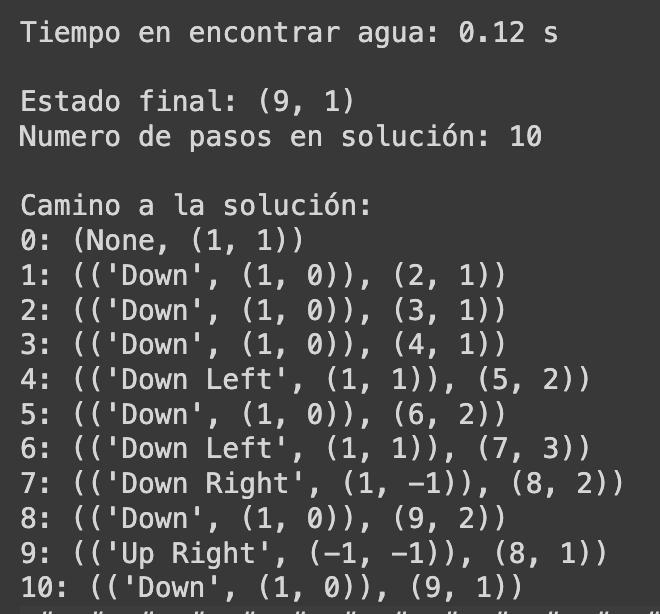
\includegraphics[scale=0.25,angle=0]{anchuram1ruta.jpeg}
                \end{subfigure}
                \hfill
                \centering
                \caption{Descripción de la ruta del \textit{Rover} en el Mapa 1 con Búsqueda por Anchura.}\label{an_m1_d}
            \end{figure}

            \begin{figure}[h!]
                \centering
                \begin{subfigure}[h!]{0.45\textwidth}
                    \centering
                    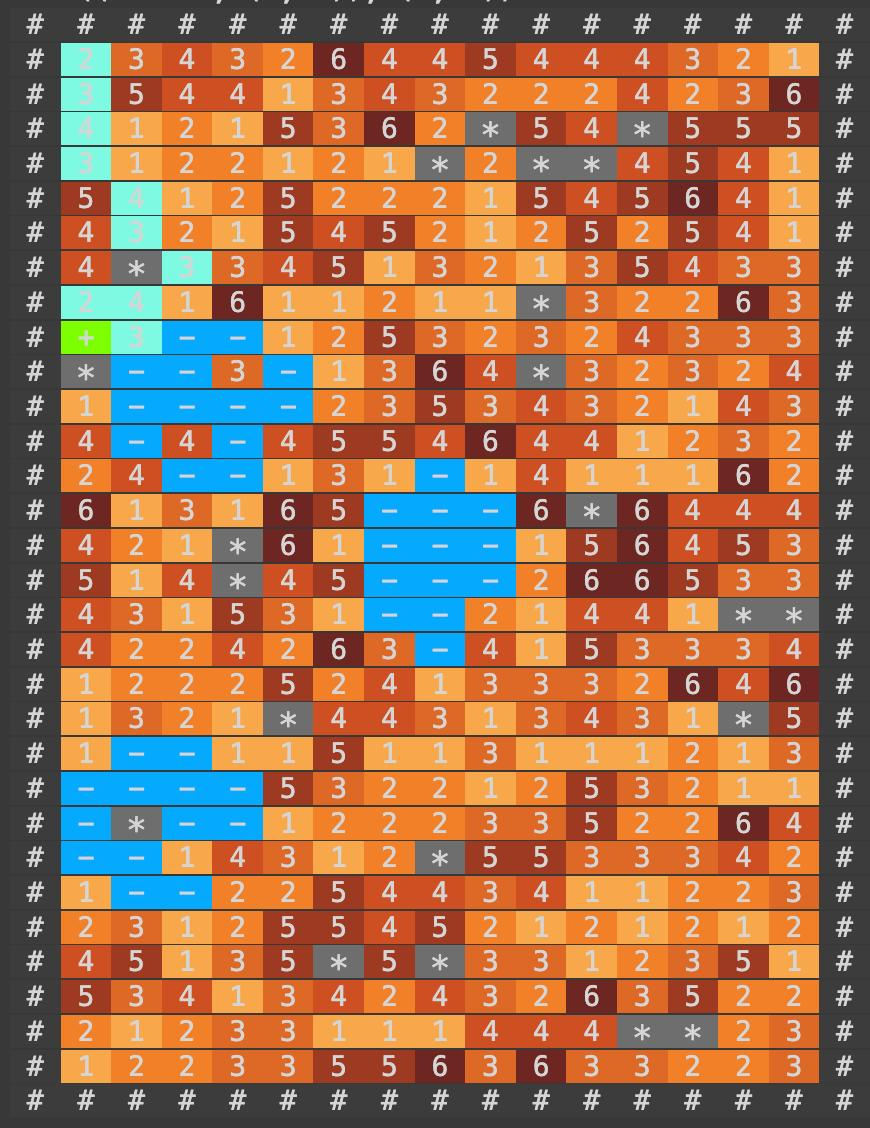
\includegraphics[scale=0.2,angle=0]{anchuram1g.jpeg}
                \end{subfigure}
                \hfill
                \centering
                \caption{Visualización de la ruta del \textit{Rover} en el Mapa 1 con Búsqueda por Anchura.}\label{an_m1_g}
            \end{figure}

        \subsubsection{Profundidad}

    \subsection{Locales}

        \subsubsection{\textit{Hill Climbing}}

            \paragraph{Altura máxima}

            \paragraph{Altura mínima}

        \subsubsection{\textit{Hill Climbing with Random Restarts}}

            \paragraph{Altura máxima}

            \paragraph{Altura mínima}

        \subsubsection{\textit{Simulated Annealing} ó Recocido Simulado}

            \paragraph{Altura máxima}

            \paragraph{Altura mínima}

\section{Análisis de Búsquedas}

    \subsection{Informadas y No Informadas}

        \subsubsection{Mapa 1}

        \subsubsection{Mapa 2}

        \subsubsection{Mapa 3}

    \subsection{Locales}

        \subsubsection{\textit{Hill Climbing}}

        \subsubsection{\textit{Hill Climbing with Random Restarts}}

        \subsubsection{\textit{Simulated Annealing} ó Recocido Simulado}

\section{Conclusiones}

\appendix

\section{Nombre del Apéndice}
% El apéndice es una sección que se añade al final del documento, después de la bibliografía, y que contiene información adicional que no es esencial para la comprensión del texto principal, pero que puede ser útil para el lector. 
% Por ejemplo, en un artículo científico, el apéndice puede contener datos experimentales adicionales, cálculos matemáticos detallados, o información técnica que no es esencial para la comprensión del artículo, pero que puede ser útil para los lectores interesados en los detalles técnicos del trabajo.

\section{Referencias}
% \begin{thebibliography}{99}

\bibliographystyle{plain}
\bibliography{pruebabib}

\end{document}